\part{Traveling Salesman Problem}
\chapter{Symmetric Traveling Salesman Problem}

\section{Problem Definition}
旅行商问题(Traveling Salesman Problem, TSP\index{TSP})是组合优化领域的经典问题之一,其核心目标是给定城市列表和每对城市之间的距离,求恰好访问每个城市一次并返回起始城市的最短可能路线。该问题于1930年正式提出,是优化中研究最深入的问题之一,被用作许多优化方法的基准。自从该问题被正式提出以来,一直是运筹学、计算机科学和物流管理等领域的研究热点,尽管该问题在计算上很困难,但许多启发式方法和精确算法是已知的\cite{2009A, 2012Models}。

\begin{figure}[!htb]
    \centering
    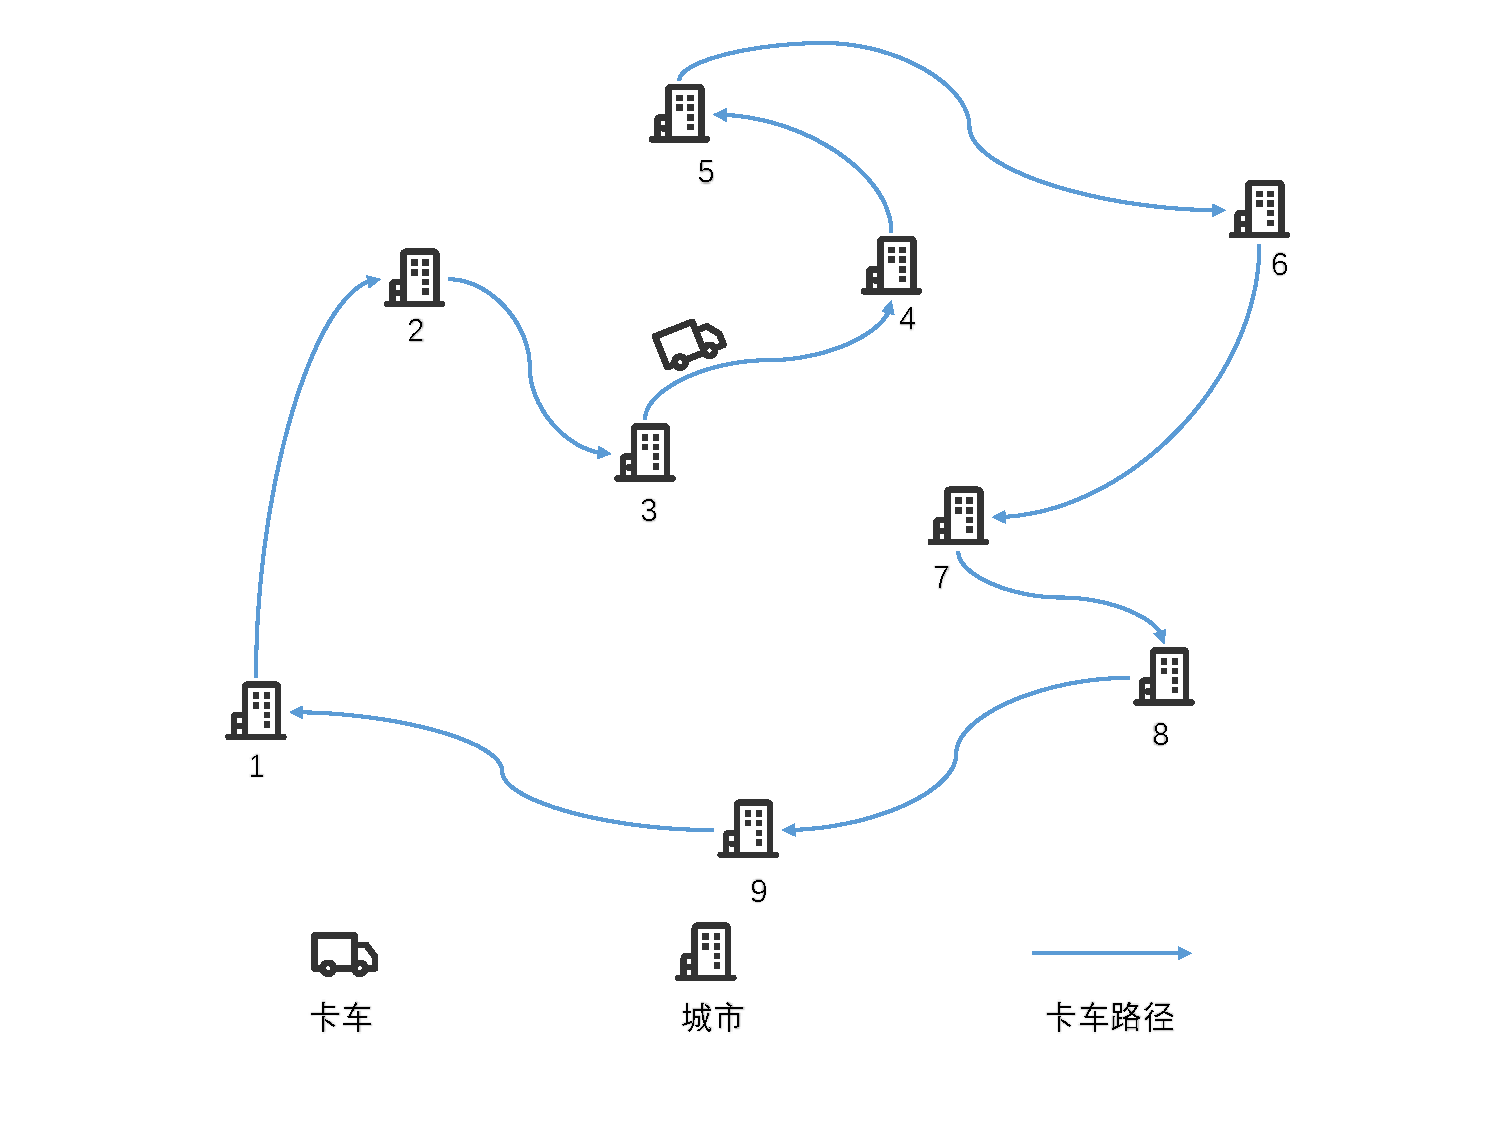
\includegraphics[width=\linewidth]{images/TSP.pdf}\\
    \caption{TSP示意图}
\end{figure}

TSP可以表述为整数线性规划模型\cite{papadimitriou1998combinatorial}:假设共有$N$个城市,每个城市的编号为$1,\cdots,N$,从城市$i$到城市$j$的旅行成本(距离)为$c_{ij}>0$。旅行商的目标是从任意一个城市出发访问完所有的城市,每个城市只能访问一次,最后回到最初的城市,目标是找到一条依次访问所有城市且访问城市不重复的最短路线。TSP中的决策变量为$x_{ij}=\begin{cases}1, & \text{存在从城市$i$到城市$j$的路径}\\0, & \text{其他} \end{cases}$,城市节点集合表示为$V(|V| = N)$。由于可能存在子回路,所以在构建TSP模型时需要消除会产生子回路的情况,这里采用Miller-Tucker-Zemlin (MTZ\index{MTZ})约束进行子回路的消除\cite{1960Integer},引入连续变量$u_i(\forall i \in V, u_i \geq 0)$,其取值可以为任何非负实数(实数集合表示为$R$)。这里用$u_i$表示编号为$i$的城市的访问次序,比如当$u_i = 5$时表示编号为1的城市是从出发点开始,第5个被访问到的点。因此,TSP的数学模型可以表示为MILP \ref{model:model-tsp}。

\begin{model}{TSP MILP}{model-tsp}
\begin{align}
    \min \quad & \sum_{i \in V}\sum_{j \in V, i \neq j} c_{ij}x_{ij} & \label{eq:tsp-obj}\\
    \text{s.t.} \quad & \sum_{i \in V} x_{ij} = 1, & \forall j \in V, i \neq j\label{eq:tsp-in}\\
    \quad & \sum_{j \in V} x_{ij} = 1, & \forall i \in V, i \neq j \label{eq:tsp-out}\\
    \quad & u_i - u_j + Nx_{ij} \leq N - 1, & \forall i, j \in V; i \neq j \label{eq:tsp-subtour}\\
    \quad & u_i \geq 0, & u_i \in R \label{eq:tsp-u_bound}\\
    \quad & x_{ij} \in \{0, 1\}, & i, j \in V; i \neq j\label{eq:tsp-x_bound}
\end{align}
\end{model}

目标函数\ref{eq:tsp-obj}表示最小化访问所有城市的成本(距离),约束\ref{eq:tsp-in}和\ref{eq:tsp-out}保证每个城市节点的入度和出度为1,即每个城市只进入一次和出去一次,保证了每个城市只访问一次,不会被重复访问,约束\ref{eq:tsp-subtour}消除子回路,约束\ref{eq:tsp-u_bound}和\ref{eq:tsp-x_bound}表示变量的取值范围。

\section{Solution Methods}

\subsection{Exact Methods}
\href{https://www.math.uwaterloo.ca/tsp/concorde/index.html}{Concorde}是一个求解TSP的精确算法,由\href{https://www.wikiwand.com/en/articles/ANSI_C}{ANSI C}编写。在\href{https://www.math.uwaterloo.ca/tsp/concorde/downloads/downloads.htm}{Concorde Download}页面可以下载到最新版本的Concorde。下载后通过在命令行输入命令\ref{code:concorde-unzip}进行解压,解压后会得到一个名为\texttt{concorde}的文件夹,编译的过程参考\href{https://www.freesion.com/article/5581560004/}{Ubuntu(Linux)安装concorde过程}或者参考\href{https://github.com/perrygeo/pytsp/wiki/Installing-Solvers}{Installing Concorde}。

\begin{code}{Concorde unzip}{concorde-unzip}
\begin{minted}{pwsh}
gunzip co031219.tgz
tar xvf co031219.tar
\end{minted}
\end{code}

Concorde需要linear programming solver,常用的有\href{https://www.math.uwaterloo.ca/~bico/qsopt/index.html}{QSOpt}和IBM的\href{https://www.ibm.com/products/ilog-cplex-optimization-studio/cplex-optimizer}{CPLEX},由于Concorde自从2003年之后就没有更新过,因此当前CPLEX的版本已经不再合适,因此选用QSOpt。QSOpt的路径假设为\mintinline{bash}{path=/home/kaiyouhu/qsopt},用命令\ref{code:qsopt-download}下载QSOpt的头文件,

\begin{code}{QSOpt download}{qsopt-download}
\begin{minted}{bash}
mkdir qsopt
cd qsopt
wget -O qsopt.a http://www.math.uwaterloo.ca/~bico/qsopt/beta/codes/PIC/qsopt.PIC.a # WSL上的Ubuntu测试有效
wget http://www.math.uwaterloo.ca/~bico/qsopt/beta/codes/linux64/qsopt.h
wget http://www.math.uwaterloo.ca/~bico/qsopt/beta/codes/linux64/qsopt
\end{minted}
\end{code}

然后在\texttt{concorde}文件夹下使用命令\ref{code:concorde-make}编译Concorde,编译完成后会在当前目录下生成一个名为\texttt{TSP}的文件。

\begin{code}{Concorde make}{concorde-make}
\begin{minted}{bash}
CFLAGS="-fPIC -O2 -g" ./configure --with-qsopt=/home/kaiyouhu/qsopt # 如果QSOpt的路径不同记得修改
# continue
make
cd TSP
./concorde -s 99 -k 100 # -s 99表示使用随机种子99,-k 100表示使用100个城市的TSP实例进行测试
\end{minted}
\end{code}

在\texttt{Python}中使用\texttt{Concorde}可以参考\href{https://github.com/jvkersch/pyconcorde}{pyconcorde},该项目是\texttt{Concorde}的\texttt{Python}接口,需要注意的是这个\texttt{Python}接口不支持\texttt{Windows}系统,但是支持\texttt{WSL},具体的安装细节\href{https://github.com/jvkersch/pyconcorde}{参考文档说明}。

\subsection{Heuristic Methods}
\href{http://akira.ruc.dk/~keld/research/LKH/}{LKH}是解决TSP的\href{https://www.wikiwand.com/en/articles/Lin%E2%80%93Kernighan_heuristic}{Lin-Kernighan}启发式算法的有效实现,基于ANSI C编写。在此之外,LKH还有一个改进的\href{http://akira.ruc.dk/~keld/research/LKH-3/}{LKH-3}版本,支持多种约束条件(Asymmetric capacitated vehicle routing problem, Multiple traveling salesmen problem, Sequential ordering problem$\dots$)的TSP求解。在\href{http://akira.ruc.dk/~keld/research/LKH/}{LKH}页面可以下载到最新版本的LKH实现代码。下载后通过在命令行输入命令\ref{code:lkh-unzip}进行解压,解压后会得到一个名为\texttt{LKH-2.0.10}的文件夹,然后在\texttt{Linux}或者\texttt{WSL}下输入命令\mintinline{bash}{make}编译LKH代码,编译完成后会在当前目录下生成一个名为\texttt{LKH}的文件。

\begin{code}{LKH unzip and make}{lkh-unzip}
\begin{minted}{pwsh}
tar xvfz LKH-2.0.10.tgz
cd LKH-2.0.10
make
\end{minted}
\end{code}

在\texttt{Python}中使用\texttt{LKH}可以参考\href{https://github.com/ntnu-arl/LKH_TSP}{LKH\_TSP},该项目是\texttt{LKH}的\texttt{Python}接口,需要注意的是这个\texttt{Python}接口不支持\texttt{Windows}系统,但是可以在\texttt{WSL}中运行。
